\documentclass[tikz,border=4pt]{standalone}
\usepackage{tikz}
\usetikzlibrary{arrows.meta}
\begin{document}
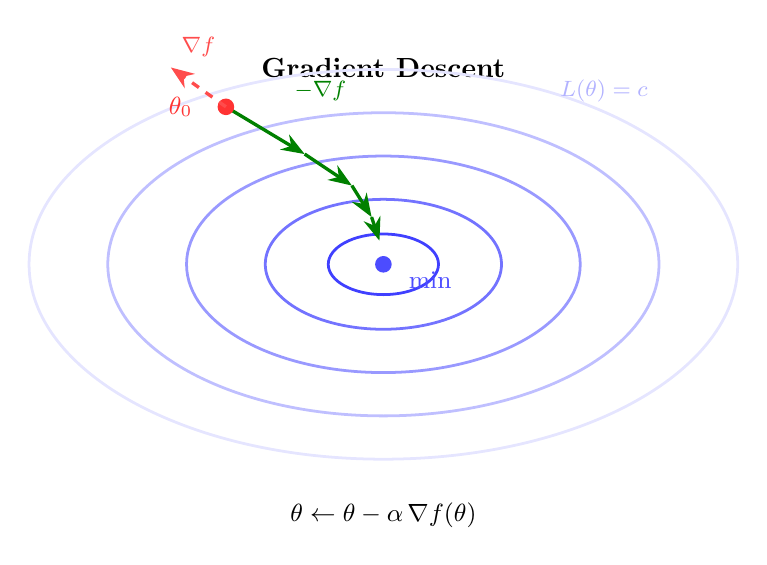
\begin{tikzpicture}[
    >=Stealth,
    vec/.style={->,line width=1.2pt},
]
\node[font=\bfseries] at (3,5.3) {Gradient Descent};

% Contour ellipses
\foreach \r/\c in {4.5/10, 3.5/25, 2.5/40, 1.5/55, 0.7/75} {
    \draw[blue!\c!white, line width=1pt]
        (3,2.8) ellipse ({\r} and {\r*0.55});
}

% Minimum point
\fill[blue!70] (3,2.8) circle (3pt);
\node[blue!70,font=\small,right] at (3.2,2.6) {min};

% Gradient descent path
\foreach \a/\b/\c/\d in {
    1.0/4.8/2.0/4.2,
    2.0/4.2/2.6/3.8,
    2.6/3.8/2.85/3.4,
    2.85/3.4/2.95/3.1} {
    \draw[vec,green!50!black] (\a,\b) -- (\c,\d);
}

% Starting point
\fill[red!80] (1.0,4.8) circle (3pt);
\node[red!80,font=\small,left] at (0.7,4.8) {$\theta_0$};

% Gradient arrow (pointing outward = uphill)
\draw[vec,red!70,dashed] (1.0,4.8) -- (0.3,5.3)
    node[above right,font=\footnotesize] {$\nabla f$};

% Negative gradient direction label
\node[green!50!black,font=\footnotesize] at (2.2,5.0)
    {$-\nabla f$};

% Contour label
\node[blue!30,font=\footnotesize] at (5.8,5.0) {$L(\theta)=c$};

% Formula
\node[font=\small,anchor=north] at (3,-0.1)
    {$\theta \leftarrow \theta - \alpha\,\nabla f(\theta)$};
\end{tikzpicture}
\end{document}
